% LTeX: language=it

\documentclass{../.common/high-school-notebook}

\hypersetup{
  pdftitle={Quaderno delle regole - Fisica},
  pdfauthor={Tommaso Bocchietti},
  pdfsubject={High School Notebook},
}

\begin{document}

\title{Quaderno delle regole - Fisica}
\author{Tommaso Bocchietti}

\maketitle

\begin{figure}[H]
    \centering
    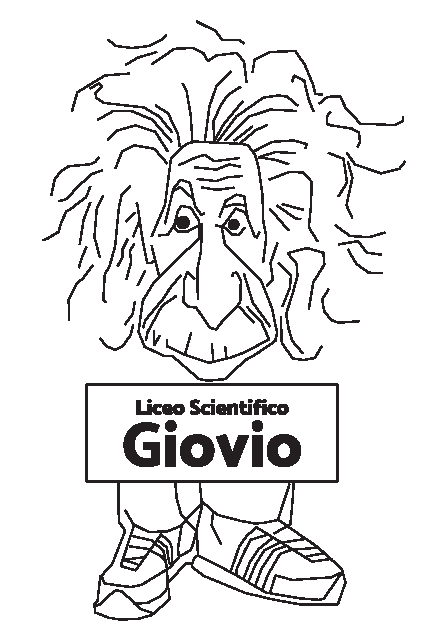
\includegraphics[width=0.7\textwidth]{../.common/Einstein_Logo}
    \label{fig:Einstein_Logo}
\end{figure}


\clearpage
\tableofcontents

% \clearpage
% % LTeX: language=it

\section{Basi della fisica}


% \clearpage
% % LTeX: language=it

\section{I moti}

% % LTeX: language=it

\section{Leggi di Newton}

% % LTeX: language=it

\section{Lavoro}


% \clearpage
% % LTeX: language=it

\section{I moti del piano}

% % LTeX: language=it

\section{Il modello standard}

% % LTeX: language=it

\section{Forza gravitazionale}

% % LTeX: language=it

\section{Quantità di moto e Momento angolare}

% % LTeX: language=it

\section{Termologia}

% % LTeX: language=it

\section{Legge dei gas}

% % LTeX: language=it

\section{Termodinamica}

% % LTeX: language=it

\section{Entropia}


\clearpage
% % LTeX: language=it

\section{Moto armonico}

% % LTeX: language=it

\section{Le onde}

% % LTeX: language=it

\section{Suono}

% % LTeX: language=it

\section{Ottica}

% % LTeX: language=it

\section{Elettrostatica}

L'elettrostatica studia le cariche elettriche stazionarie nel tempo.
Gli elettroni hanno massa $m_e = \SI{9.109e-31}{\kilo\gram}$ e carica negativa.
I protoni hanno massa $m_p = \SI{1.673e-27}{\kilo\gram}$ e carica positiva.
La carica elementare equivale a $e = \SI{1.602e-19}{\coulomb}$.

Un corpo si dice isolante se i suoi elettroni sono dissi e impossibilitati a muoversi, ma solo direzionarsi.
É un conduttore se gli elettroni sono liberi di muoversi e spostarsi.

\subsection{Legge di Coulomb}

Per il calcolo della forza tra due cariche puntiformi si usa la legge di Coulomb:

\begin{equation*}
    F = k_0 \frac{Q_1 Q_2}{r^2}
\end{equation*}

Dove $k_0 = \frac{1}{4\pi\varepsilon_0}$, con $\varepsilon_0 = \text{Costante dielettrica del vuoto} = \SI{8.854e-12}{\coulomb\squared\per\newton\per\meter\squared}$.

I materiali si possono caricare per strofinio, contatto o induzione. Gli isolanti, o dielettrici, si possono solo polarizzare (polarizzazione).

Costante dielettrica relativa $\varepsilon = \varepsilon_r \varepsilon_0$.

\subsection{Il campo elettrico}

Un campo vettoriale è una funzione che associa a ogni punto dello spazio, un vettore che specifica in modulo, direzione e verso, una data grandezza vettoriale.

Forza generata da un campo elettrico:

\begin{equation*}
    \vec{F} = q \vec{E} \rightarrow \SI{}{\newton} = \SI{}{\coulomb} \cdot \frac{\SI{}{\newton}}{\SI{}{\coulomb}}
\end{equation*}

Dove $q = \text{carica di prova}$.

Rappresentazione grafica:

% TODO: carica elettrica con linee di campo
% TODO: dipolo elettrico con linee di campo

\subsection{Flusso del campo elettrico / Teorema di Gauss}

\begin{align*}
    \text{Per superfici aperte}: & \Phi_S(\vec{E}) = \int_S \vec{E} \cdot \vec{S} \, dS = \sum_{i = 1}^{N} \vec{E_i} \cdot \vec{\Delta S_i}            \\
    \text{Per superfici chiuse}: & \Phi_\Omega(\vec{E}) = \frac{Q_{tot}}{\varepsilon}, \text{con } Q_{tot} = \text{carica totale contenuta in } \Omega
\end{align*}

% TODO: esempio di superficie aperta
% TODO: esempio di superficie chiusa con carica interna

\subsection{Forme di campo elettrico in casi noti}

Ipotizzando di essere nel vuoto, e quindi di avere $\varepsilon = \varepsilon_0$, possiamo dare la definizione di $\vec{E}$ per alcuni casi particolari.

\begin{itemize}
    \item Carica puntiforme: $\vec{E} = k_0 \frac{Q}{r^2} \hat{r}$
    \item Piano infinito uniformemente carico: $\vec{E} = \frac{\sigma}{2\varepsilon_0} \hat{n}$, con $\sigma = \text{densità di carica superficiale} \SI{}{\coulomb\per\meter\squared}$
    \item Filo infinito uniformemente carico: $\vec{E} = \frac{\lambda}{2\pi\varepsilon_0 r} \hat{r}$, con $\lambda = \text{densità di carica lineare} \SI{}{\coulomb\per\meter}$ e $r = \text{distanza dal filo}$
    \item Una sfera, al suo esterno: $\vec{E} = k_0 \frac{Q}{r^2} \hat{r}$ (essenzialmente una carica puntiforme)
    \item Una sfera conduttrice, al suo interno: $\vec{E} = 0$ perché le cariche si distribuiscono sulla superficie
    \item Una sfera dielettrica, al suo interno: $\vec{E} = r \cdot k_0 \frac{Q}{R^3} \hat{r}$, con $Q = \text{carica compresa nel volume di raggio} r$
    \item In un condensatore piano: $\vec{E} = \frac{\sigma}{\varepsilon_0}$. All'esterno delle barriere, $\vec{E} = 0$
\end{itemize}

\subsection{Energia potenziale elettrica}

L'energia potenziale elettrica tra due cariche puntiformi è:

\begin{equation*}
    U = k_0 \frac{Q_1 Q_2}{r}
\end{equation*}

% TODO: grafico dell'energia potenziale elettrica caso >0 e caso <0

In generale: $U = L = \vec{F} \cdot \vec{s} = q \vec{E} \cdot \text{distanza dalla fonte di campo}$

\subsection{Potenziale elettrico}

Il potenziale elettrico è una funzione scalare che associa a ogni punto dello spazio un valore scalare che specifica l'energia potenziale elettrica di una carica di prova $q$ in quel punto.

\begin{equation*}
    V = \frac{U}{q} = \frac{L}{q} = \frac{\vec{F} \cdot \vec{s}}{q} = \vec{E} \cdot \vec{s}
\end{equation*}

In generale, definito $\Delta V = V_B - V_A$ differenza di potenziale, si ha:

\begin{equation*}
    \Delta V = -\vec{E} \cdot \Delta \vec{s} \rightarrow L = U_A - U_B = - q \Delta V
\end{equation*}

Partendo quindi da $U_{A \rightarrow B} = -q \Delta V = -q (V_B - V_A)$, abbiamo che il lavoro è positivo, e quindi le cariche si spostano autonomamente, se la carica $q$ è:

\begin{itemize}
    \item Positiva, e allora passa da potenziale maggiore a potenziale minore $\rightarrow$ $V_A > V_B$
    \item Negativa, e allora passa da potenziale minore a potenziale maggiore $\rightarrow$ $V_A < V_B$
\end{itemize}

% TODO: schemino di una carica immersa in un campo elettrico con valutazioni su V U e L

Una superficie equipotenziale è il luogo dei punti dello spazio aventi lo stesso potenziale elettrico.

Un esempio è il condensatore piano, che forma tra le sue armature una serie di superfici equipotenziali.

\begin{figure}[H]
    \centering
    \begin{tikzpicture}

        % Draw walls
        \draw[line width=2mm] (0,0) -- (0,3);
        \draw[line width=2mm] (5,0) -- (5,3);

        % Draw electric field lines
        \foreach \y in {0.5,1.5,2.5}
        \draw[postaction={
                    decorate,
                    decoration={
                            markings,
                            mark=between positions 0.2 and 1 step 1.5cm with {\arrow{latex}}
                        }}] (0,\y) -- (4.9,\y);

        % Draw equipotential lines
        \foreach \x in {1.5,3.5}
        \draw[dashed, color=red] (\x, 0) -- (\x,3);

        % Draw equipotential lines
        \foreach \y in {0.5,1,...,2.5}
            {
                \node at (-0.5,\y) {+};
                \node at ( 5.5,\y) {-};
            }
    \end{tikzpicture}
    \caption{Condensatore piano con \textcolor{red}{superfici equipotenziali}}
\end{figure}

\subsection{Circuitazione del campo elettrico lungo una linea chiusa orientata}

É una legge che serve per dimostrare che il campo elettrico $\vec{E}$, rimane costante ed è quindi conservativo.

\begin{equation*}
    \oint_\mathcal{L} \vec{E} = \sum_{i = 1}^{n} \vec{E} \cdot \vec{\Delta s_i}
\end{equation*}

Visto che il campo elettrico è conservativo, deve valere che $\oint_\mathcal{L} \vec{E} = 0$ sempre, ammesso che la linea $\mathcal{L}$ sia chiusa.

\subsection{Distribuzione delle cariche nei conduttori}

Le cariche tendono sempre a mettersi sulle superfici esterne.
L'interno dunque di un conduttore rimane con $\vec{E} = 0$, e $V_{interna} = V_{superficie}$ e dunque $\Delta V = 0$.

Il potere delle punte è un fenomeno correlato alla distribuzione delle cariche sui conduttori per cui si ha $S_{punta} \approx 0$ e quindi $\vec{E} = \frac{Q}{S\varepsilon} = \infty$.
Da questo ne deriva che alcuni cariche possono essere espulse dal conduttore generando così un vento elettrico.

\subsection{Teorema di Coulomb}

Per calcolare il campo elettrico sulla superficie di un conduttore si ha $\vec{E} = \frac{\sigma}{\varepsilon}$

% TODO: disegno conduttore con superficie elettrizzata

\subsection{Capacità di un condensatore}

É definita come il rapporto tra la carica elettrica e il potenziale elettrico:

\begin{equation*}
    C = \frac{Q}{V} \SI{}{\farad} = \SI{}{\coulomb\per\volt}
\end{equation*}

Corrisponde alla quantità di carica che può contenere un conduttore.

\begin{itemize}
    \item Per una sfera conduttrice: $C = 4\pi\varepsilon_0 R$
    \item Per un condensatore piano: $C = \varepsilon_0 \frac{S}{d}$, con $S = \text{superficie delle armature}$ e $d = \text{distanza tra le armature}$
\end{itemize}

\subsection{Energia immagazzinata in un condensatore}

Corrisponde al lavoro compiuto per caricare il condensatore

\begin{equation*}
    W_c = \frac{1}{2} \frac{Q^2}{C} = \frac{1}{2} C V \SI{}{\joule}
\end{equation*}

\subsection{Densità di energia in un condensatore}

É il rapporto tra l'energia immagazzinata e il volume del condensatore tra le pareti.

\begin{equation*}
    w_{\vec{E}} = \frac{W_c}{Sd} = \frac{1}{2} \varepsilon_0 E^2 \SI{}{\joule\per\meter\cubed}
\end{equation*}

\subsection{Proprietà fondamentali del campo elettrico}

Si riportano qui le due proprietà fondamentali del campo elettrico:

\begin{itemize}
    \item Flusso del campo elettrico da una superficie chiusa: $\Phi_\Omega(\vec{E}) = \frac{Q_{tot}}{\varepsilon}$
    \item Circuitazione del campo elettrico lungo una linea chiusa orientata: $\oint_\mathcal{L} \vec{E} = 0$
\end{itemize}























% % LTeX: language=it

\section{Corrente elettrica}


\clearpage
% % LTeX: language=it

\section{Campo magnetico}

% % LTeX: language=it

\section{Corrente indotta}

\subsection{Legge di Faraday-Neumann}

\subsection{Legge di Lenz}

\subsection{Correnti di Foucault}
% LTeX: language=it

\section{Induttanza}

% % LTeX: language=it

\section{Corrente alternata}

% % LTeX: language=it

\section{Equazioni di Maxwell}

Nel 1865, Maxwell comprese che il campo elettrico e il campo magnetico si influenzavano reciprocamente.
Egli propose delle equazioni basate sul flusso e sulla circuitazione di $\vec{E}$ e $\vec{B}$ per dimostrarlo.

\subsection{Circuitazione di $\vec{E}$ lungo $\mathcal{L}$}

Partendo da $\oint_{\mathcal{L}} \vec{E} = 0$, Maxwell dimostrò che tale circuitazione è legata alla forza elettromotrice $\text{fem}(\vec{B})$ attraverso:

\begin{equation*}
    \oint_{\mathcal{L}} \vec{E} = - \frac{\Delta \Phi_S(\vec{B})}{\Delta t}
\end{equation*}

Questo indica che un campo elettrico può essere generato da cariche elettriche o da campi magnetici variabili nel tempo.

\subsection{Circuitazione di $\vec{B}$ lungo $\mathcal{L}$}

Partendo da $\oint_{\mathcal{L}} \vec{B} = \mu_0 \cdot I_{\text{concatenata}}$, Maxwell introdusse la corrente di spostamento $I_s = \varepsilon_0 \cdot \frac{\Delta \Phi_S(\vec{E})}{\Delta t}$.
Quindi, la circuitazione diventa:

\begin{equation*}
    \oint_{\mathcal{L}} \vec{B} = \mu_0 \cdot \left( I_c + I_s \right) = \mu_0 \cdot \left( I_c + \varepsilon_0 \cdot \frac{\Delta \Phi_S(\vec{E})}{\Delta t} \right)
\end{equation*}

Questo dimostra che un campo magnetico può essere generato da correnti elettriche o da campi elettrici variabili nel tempo.

\subsection{Definizione di campo elettromagnetico}

La combinazione delle equazioni di Maxwell porta alla definizione del campo elettromagnetico, in cui $\vec{E}$ e $\vec{B}$ si influenzano reciprocamente senza la necessità di un mezzo materiale.

\begin{align*}
    \Phi_\Omega(\vec{E})        & = \frac{Q_{\text{tot}}}{\varepsilon}                                                           \\
    \Phi_\Omega(\vec{B})        & = 0                                                                                            \\
    \oint_{\mathcal{L}} \vec{E} & = - \frac{\Delta \Phi_S(\vec{B})}{\Delta t}                                                    \\
    \oint_{\mathcal{L}} \vec{B} & = \mu_0 \cdot \left( I_c + \varepsilon_0 \cdot \frac{\Delta \Phi_S(\vec{E})}{\Delta t} \right)
\end{align*}

La risoluzione di queste equazioni conduce alla definizione delle onde elettromagnetiche, come ad esempio la luce.

% % LTeX: language=it

\section{Onde elettromagnetiche}

\begin{figure}[H]
    \centering

    % https://tikz.net/electromagnetic_wave/
    % Electromagnetic wave - colored
    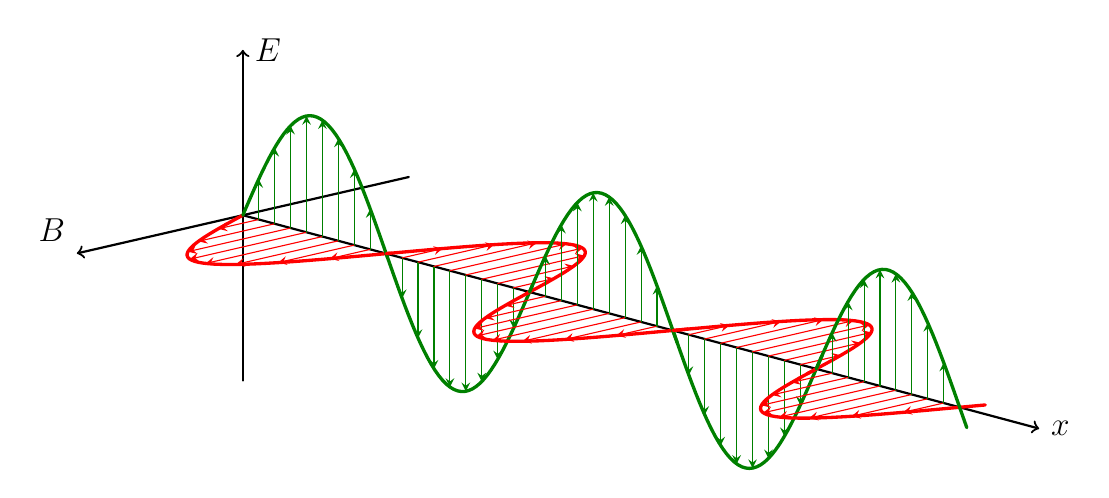
\begin{tikzpicture}[x=(-15:1.2), y=(90:1.0), z=(-150:1.0),
            line cap=round, line join=round,
            axis/.style={black, thick,->},
            vector/.style={>=stealth,->}]
        \large
        \def\A{1.5}
        \def\nNodes{5} % use even number
        \def\nVectorsPerNode{8}
        \def\N{\nNodes*40}
        \def\xmax{\nNodes*pi/2*1.01}
        \pgfmathsetmacro\nVectors{(\nVectorsPerNode+1)*\nNodes}

        \def\drawENode{ % draw E node and vectors with some offset
            \draw[Green,very thick,variable=\t,domain=\iOffset*pi/2:(\iOffset+1)*pi/2*1.01,samples=40]
            plot (\t,{\A*sin(\t*360/pi)},0);
            \foreach \k [evaluate={\t=\k*pi/2/(\nVectorsPerNode+1);
                        \angle=\k*90/(\nVectorsPerNode+1);}]
            in {1,...,\nVectorsPerNode}{
                    \draw[vector,Green]  (\iOffset*pi/2+\t,0,0) -- ++(0,{\A*sin(2*\angle+\iOffset*180)},0);
                }
        }
        \def\drawBNode{ % draw B node and vectors with some offset
            \draw[Red,very thick,variable=\t,domain=\iOffset*pi/2:(\iOffset+1)*pi/2*1.01,samples=40]
            plot (\t,0,{\A*sin(\t*360/pi)});
            \foreach \k [evaluate={\t=\k*pi/2/(\nVectorsPerNode+1);
                        \angle=\k*90/(\nVectorsPerNode+1);}]
            in {1,...,\nVectorsPerNode}{
                    \draw[vector,Red]  (\iOffset*pi/2+\t,0,0) -- ++(0,0,{\A*sin(2*\angle+\iOffset*180)});
                }
        }

        % MAIN AXES
        \draw[axis] (0,0,0) -- ++(\xmax*1.1,0,0) node[right] {$x$};
        \draw[axis] (0,-\A*1.4,0) -- (0,\A*1.4,0) node[right] {$E$};
        \draw[axis] (0,0,-\A*1.4) -- (0,0,\A*1.4) node[above left] {$B$};

        % draw (anti-)nodes
        \foreach \iNode [evaluate={\iOffset=\iNode-1;}] in {1,...,\nNodes}{
                \ifodd\iNode \drawBNode \drawENode % E overlaps B
                \else        \drawENode \drawBNode % B overlaps E
                \fi
            }

    \end{tikzpicture}
    \caption{Onda elettromagnetica}
\end{figure}



% % LTeX: language=it

\section{Spettro elettromagnetico}

L'ampio spettro elettromagnetico comprende un insieme di frequenze delle onde elettromagnetiche, ognuna con caratteristiche specifiche.
Questo spettro può essere suddiviso in sette categorie principali, ciascuna con una gamma di lunghezze d'onda distintiva.

\begin{figure}[H]
    \centering
    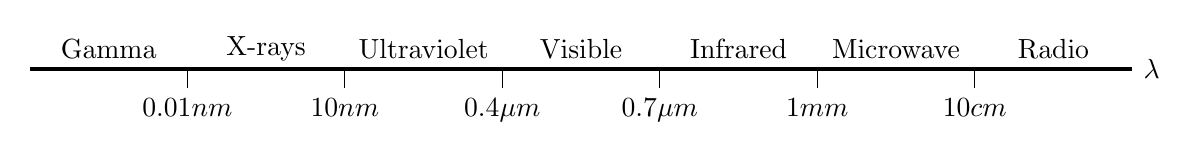
\begin{tikzpicture}[scale=0.5]
        % Spectrum lines
        \draw[ultra thick] (0,0) -> (28,0) node[right] {$\lambda$};

        % Wavelengths
        \foreach \w/\label in {4/$0.01nm$, 8/$10nm$, 12/$0.4\mu m$, 16/$0.7\mu m$, 20/$1mm$, 24/$10cm$}
            {
                \draw (\w,0) -- (\w,-0.5) node[below] {\label};
            }

        % Labels
        \foreach \w/\label in {2/Gamma, 6/X-rays, 10/Ultraviolet, 14/Visible, 18/Infrared, 22/Microwave, 26/Radio}
            {
                \node at (\w, 0.5) {\label};
            }

        % % Rainbow-colored band in the visible region (between 12 and 16)
        % \fill[red] (12,0) rectangle (12.8,0.2);
        % \fill[orange] (12.8,0) rectangle (13.6,0.2);
        % \fill[yellow] (13.6,0) rectangle (14.4,0.2);
        % \fill[green] (14.4,0) rectangle (15.2,0.2);
        % \fill[cyan] (15.2,0) rectangle (16,0.2);

    \end{tikzpicture}
    \caption{Spettro elettromagnetico}
\end{figure}

Con la conoscenza della lunghezza d'onda, è possibile calcolare la frequenza dell'onda elettromagnetica utilizzando la formula $f = \frac{c}{\lambda}$, in cui $c$ rappresenta la velocità della luce.
Un'importante porzione dello spettro è la luce visibile, con lunghezze d'onda comprese tra $400nm$ (viola) e $700nm$ (rosso).
Questa fascia visibile è cruciale per la percezione umana dei colori, spaziando attraverso l'interessante intervallo di colori che va dal viola al rosso.
% % LTeX: language=it

\section{Relatività ristretta}

\subsection{Velocità della luce e sistemi di riferimento}

\subsection{L'esperimento di Michelson-Morley (1887)}

\subsection{Gli assiomi della teoria della relatività ristretta}

\subsection{La simultaneità}

\subsection{La dilatazione dei tempi}

\subsection{La contrazione delle lunghezze}

\subsection{L'invarianza delle lunghezze perpendicolari al moto relativo}

\subsection{Le trasformazioni di Lorentz}

\subsection{L'intervallo invariante}

\subsection{Lo spazio-tempo di Minkowski}

\subsection{La composizione relativistica delle velocità}

\subsection{L'equivalenza tra massa ed energia}

\subsection{La dinamica relativistica}

% % LTeX: language=it

\section{Relatività generale}



\end{document}